\documentclass[11pt]{article}
\usepackage[margin=1.05in]{geometry}
\usepackage[T1]{fontenc}
\usepackage[utf8]{inputenc}
\usepackage{lmodern}
\usepackage{amsmath,amssymb,amsthm}
\usepackage{booktabs,array,longtable}
\usepackage{graphicx}
\usepackage{microtype}
\usepackage{tikz}
\usetikzlibrary{arrows.meta,positioning,calc}
\usepackage[colorlinks=true,allcolors=black,linkcolor=black,citecolor=black,
            urlcolor=blue]{hyperref}

\theoremstyle{plain}
\newtheorem{theorem}{Theorem}[section]
\newtheorem{proposition}[theorem]{Proposition}
\newtheorem{lemma}[theorem]{Lemma}
\newtheorem{corollary}[theorem]{Corollary}
\theoremstyle{definition}
\newtheorem{definition}[theorem]{Definition}
\newtheorem{example}[theorem]{Example}
\theoremstyle{remark}
\newtheorem{remark}[theorem]{Remark}

\newcommand{\R}{\mathbb{R}}
\newcommand{\N}{\mathbb{N}}
\newcommand{\E}{\mathbb{E}}
\newcommand{\one}{\mathbf{1}}
\newcommand{\Bin}{\mathrm{Bin}}
\newcommand{\leanref}[1]{{\normalfont\sffamily\footnotesize[\,#1\,]}}
\newcommand{\Scale}{S}
\setlength{\emergencystretch}{2.5em}

\hypersetup{pdftitle={The material and kinetic cost of productive chemical
memory: exact frontiers for support and proportion encodings},pdfauthor={}}

\title{\bfseries The material and kinetic cost of productive chemical memory:\\
exact frontiers for support and proportion encodings}

\author{}
\date{17 September 2026}

\begin{document}
\maketitle

\begin{abstract}
A chemical system that is to be called heritable must do two things on one
probability law: make fresh product before a deadline, and hand its own
identity to \emph{both} of the compartments it divides into. We fix a single
finite protocol --- run a batch of $K$ material units to time $T$, harvest all
product, allocate every intact molecule by one complementary coin, refill both
daughters --- and ask what that joint event costs in material, for two ways of
encoding the stored identity.

For \emph{support} memory, where the identity is which of two species is
present, we study an explicit reversible binding network with elementary
bimolecular steps. The least material budget that guarantees a quota of four
fresh product units and two memory-bearing daughters with probability
$0.999$, uniformly over all $287$ admitted preparations and over an entire
factor-two band of release rates, is exactly $32$. The certificate is a
rowwise minimum of endpoint transition kernels evaluated in exact integer
arithmetic; it needs no monotonicity in budget, deadline or rate. We then
enlarge the uncertainty: the same minimum $32$ survives allocation bias
$\theta\in[0.39,0.61]$ and a simultaneous independent multiplicative
perturbation of every one of the six rate constants by $\pm1/300$. We also
exhibit a direction in which it genuinely breaks. Untying the two exit
channels of the bound complex --- so that dissociation and product release no
longer share one rate --- excludes $K=32$ by an exact upper certificate and
raises the exact minimum to $42$. The guarantee is \emph{not} monotone in the
product-release rate: doubling release alone also breaks it, because the
dissociation channel is what returns food to the pool that replication needs
to build carriers.

For \emph{proportion} memory, where both species are always present and the
identity is the majority, no elementary network is known. We give a cooperative
gate of reaction order $229$ using $415$ units, and show
that the gate's reachable class collapses to two states, which makes the whole
architecture class exactly optimisable. Sharpening the partition estimate from a
union bound to an exact endpoint minimum raises its guarantee from $0.9995$ to
$0.9997$ per cycle and from $0.995$ to $0.997$ over ten. More importantly,
we compute the class's exact frontier: $253$ core units suffice at the same
specification and no member of the class does better, so that construction is
not optimal. At the support-memory specification the frontier is
$230$ core units. Because a formal gate may use unbounded reaction order and
unbounded rate constants, this is a lower bound on every such realisation:
\textbf{proportion memory costs at least $231$ units where support memory
costs $32$.} Across five decades the frontier obeys $N\approx33.3\ln(1/\delta)$;
we prove $N=q+\Theta(\log(1/\delta))$ and identify the balance law behind the
constant, in which the corridors of $m$ ordered levels have costs $4k^2z^2$
and the total grows cubically in $m$.

Concrete minima are conventional exact computer-assisted theorems; the kernel
envelope, source conservation, rate bounds, the complementary-binomial event
and the exact tail arithmetic are verified in Lean~4 against Mathlib. This is
not an end-to-end formalisation of either probability theorem, and neither
network is an experimentally calibrated chemistry.
\end{abstract}

\noindent\textbf{Keywords.} chemical heredity; finite-count stochastic
reaction networks; random partitioning; robust Markov models; exact
certificates; formal verification.

\medskip
\noindent\textbf{MSC 2020.} 60J28, 92C42, 92E20, 68V20, 60J80.

\tableofcontents

\section{Introduction}

\subsection{Producing and inheriting are one event}

A chemical system is often called heritable when its state persists, and
called productive when it converts food into something useful. Either property
alone is comparatively cheap. A catalyst that is never consumed persists
trivially; a reaction that consumes food makes product trivially. The
interesting object is a system that does both \emph{at once, out of the same
finite material}, and then divides, and is still both afterwards --- in both
halves.

That conjunction is what we charge for here. The requirements interfere. Food
spent on product is food not spent on carriers, and carriers are what the
division stage needs, because a daughter that receives no carrier has lost the
program whatever the batch produced. Conversely a preparation rich in carriers
is poor in food and may miss its output deadline. The tension is not visible
in any calculation that treats production and inheritance separately and
multiplies the answers, and it is not visible in a stationary calculation at
all, because the deadline is what makes it bite.

\subsection{Two encodings of the same bit}

Fix the simplest nontrivial memory: one bit, two programs. There are two
qualitatively different ways for finite chemistry to hold it.

\emph{Support memory.} Species $X$ is present and $Y$ is absent, or the
reverse. The decoder is a presence test. Absence is dynamically stable here
because nothing in the network creates $Y$ from an $X$-only state, so the bit
cannot flip; what can fail is that a daughter receives no molecule at all.

\emph{Proportion memory.} Both $X$ and $Y$ are always present and the bit is
which is in the majority --- whether $x/(x+y)>1/2$. This is the compositional
form of heredity studied since \cite{segre2000}, and it is strictly harder in
a specific finite-count sense: a daughter must receive a count \emph{inside a
corridor}, not merely a nonzero count, and the corridor must be re-entered
after every division.

The two encodings are usually compared rhetorically. We compare them
numerically, on one protocol, at one specification, and the gap turns out to
be large and to have an identifiable source.

\subsection{Contributions}

\begin{enumerate}\itemsep3pt
\item \textbf{A common framework} (\S\ref{sec:framework}) in which a batch,
its deadline, its harvest, one complementary allocation, and the refill that
returns both daughters to the restart set are a single probability law with a
single material ledger, and repetition along a lineage is an inequality for a
substochastic kernel rather than an independence assumption.

\item \textbf{Encoding-independent obstructions} (\S\ref{sec:obstructions}).
A carrier ceiling $K\ge q+m\lceil1+\log_2(1/\delta)\rceil$ for $m$
memory-bearing types; a first-enabling clock bound $p_*\le1-e^{-a(z)T}$ showing
that material cannot buy time, with the corollary $k\,K^{r}T\ge\log(1/\delta)$
that makes reaction order and material explicit substitutes; and, for
corridor-based memory, the necessity of $l\le g\le u$.

\item \textbf{The support-memory frontier} (\S\ref{sec:support}). The exact
robust minimum $32$, reproduced here from an independent implementation
(Theorem~\ref{thm:min32}); enlarged robustness to allocation bias and to a
simultaneous rate-constant box (\S\ref{sec:enlarged}); and a genuine failure
direction --- untying the complex's two exit channels raises the exact minimum
to $42$ (Theorem~\ref{thm:min42}) and makes the guarantee non-monotone in the
product-release rate, for a reason we identify (\S\ref{sec:branching}).

\item \textbf{The proportion-memory frontier} (\S\ref{sec:proportion}). An
endpoint reduction lemma (Lemma~\ref{lem:endpoint}) that replaces a
$7\,467$-state partition computation by four binomial evaluations; sharpened
constants for $\mathcal{R}$; and the exact minimum
over the whole cooperative-gate class --- $253$ core units at that
construction's own specification (Theorem~\ref{thm:frontier}), together with
its reliability scaling and the cascade law behind it
(\S\ref{sec:scaling}).

\item \textbf{The comparison} (\S\ref{sec:compare}). At one specification,
support memory is achieved with $32$ units by elementary bimolecular
chemistry, while proportion memory needs at least $231$ from \emph{every}
member of the cooperative-gate class, however large its reaction order and
rate constants.
\end{enumerate}

\subsection{Evidence classes}\label{sec:evidence}

We label every assertion.

\begin{itemize}\itemsep2pt
\item[\textbf{C}] a conventional mathematical proof, written out here;
\item[\textbf{E}] exact finite arithmetic over $\mathbb{Z}$ or $\mathbb{Q}$,
executed by a program whose soundness is proved in \textbf{C};
\item[\textbf{K}] a statement compiled in Lean~4 against Mathlib, with a strict
receipt (exit zero, warnings as errors, axiom report);
\item[\textbf{N}] a floating-point diagnostic or a simulation. No \textbf{N}
computation is an input to any theorem below.
\end{itemize}

Both concrete frontiers are \textbf{C/E}. The kernel-envelope inequalities,
source conservation, the daughter-return and refill identities, the rate
bounds, the complementary-binomial event identity and the exact endpoint tail
arithmetic are \textbf{K}; \S\ref{sec:lean} gives the declaration map and says
precisely where the formal boundary lies. We do not claim an end-to-end formal
proof of either probability theorem.

\subsection{What is not claimed}

Neither network is calibrated chemistry: rate constants and the deadline are
constructed benchmark values, and $T=5$ is in model time units, not seconds.
Harvest, allocation, refill and volume reset are ideal external operations;
the apparatus, the solvent, and the work of separation are excluded from the
molecular ledger, and one fuel token is a material count, not a quantity of
chemical work. The frontiers are minima \emph{within declared architecture
classes}, not universal laws about chemical memory: correlated partitioning,
multi-carrier complexes, post-division repair, other encodings and external
supplies all change the hypotheses. We make no priority claim for chemical
heredity, for programmable autocatalysis, or for robust Markov operators;
\S\ref{sec:prior} states the relation to the established literature on each.

\subsection{Relation to prior work}\label{sec:prior}

Random partitioning of molecules at division, including the effect of
complexes that partition as units, is established prior art \cite{huh2011}.
Resource-limited cellular sensing already separates copies, time and fuel as
distinct currencies \cite{govern2014}; our event is productive copying into
two actual daughters rather than sensing precision or energy per bit.
Transient loading of a module by its downstream load is the subject of
retroactivity theory \cite{delvecchio2008}; the load here is four units of
food that become product and therefore cannot become carriers. Compositional
heredity and selection in compartmentalised autocatalytic networks are studied
in \cite{segre2000,matsubara2026}, programmable autocatalytic responses in
\cite{kriukov2024}, and stochastic majority computation by low-order chemical
reaction networks in \cite{condon2020} --- the last is exactly the elementary
mechanism that our proportion-memory gate does \emph{not} provide. Structural
bounds in maximal-flux regimes \cite{despons2023} and product-form stationary
laws \cite{anderson2010} concern hypotheses different from a finite-time
chance constraint.

Methodologically, robust sets of finite-state continuous-time Markov models
with partially specified parameters, lower transition operators, and numerical
schemes with guaranteed error bounds are a developed subject
\cite{krak2017,erreygers2017}. The envelope of \S\ref{sec:envelope} is a
specialisation of that idea to one explicit chemical source, combined with
one-sided integer arithmetic; we claim the source-bound frontier and its
transparent certificate, not the operator idea.

\section{The common framework}\label{sec:framework}

\subsection{Batch, deadline, harvest, allocation, refill}

\begin{definition}[Protocol]\label{def:protocol}
A \emph{cycle} consists of the following five ideal operations.
\begin{enumerate}\itemsep1pt
\item[(P1)] \textbf{Batch.} A finite continuous-time Markov chain with
generator $G$ on a finite state space determined by a conserved material pool
of $K$ units runs from an admitted restart state $z$ for time $T$.
\item[(P2)] \textbf{Harvest.} All terminal product is collected and removed.
\item[(P3)] \textbf{Allocation.} Every remaining intact molecule is assigned
to daughter $A$ independently with probability $\theta$ (the fair case is
$\theta=1/2$); daughter $B$ receives the complement of that \emph{same} draw.
Bound complexes are allocated as single objects.
\item[(P4)] \textbf{Refill.} Each daughter's food pool is topped up to the
core mass and any consumed fuel token is replaced.
\item[(P5)] \textbf{Restart.} Both daughters are required to lie in the
restart set; one of them, designated before any randomness, continues.
\end{enumerate}
No carrier is added, removed, sorted or selected, and there is no
post-division repair. The operation is the same for every state and every
program, including after failure.
\end{definition}

Write $\mathcal{B}$ for the restart set and $q$ for the product quota. The
\emph{joint success payoff} at a terminal state is
\begin{equation}\label{eq:payoff}
h_q(z)=\one\{\,\text{product}\ge q\,\}\cdot s_\theta(z),
\end{equation}
where $s_\theta(z)$ is the conditional probability that the allocation (P3)
returns both daughters to $\mathcal{B}$. The exact one-cycle probability from
$z$ is $(e^{TG}h_q)(z)$, and the quantity to be certified is
\begin{equation}\label{eq:pstar}
p_*=\min_{z\in\mathcal{B}}\ (e^{TG}h_q)(z),
\end{equation}
the worst admitted preparation. Note that \eqref{eq:payoff} is a
\emph{single} payoff on a single law: output and inheritance are never
computed as separate marginals and multiplied.

\subsection{The two payoffs used here}

Both encodings instantiate $s_\theta$ explicitly.

For support memory, the only way a daughter fails is to receive no
carrier-bearing object at all. Conditional on $R\ge1$ such objects, the two
all-to-one-daughter events are disjoint, so
\begin{equation}\label{eq:sfair}
s_\theta(R)=1-\theta^{R}-(1-\theta)^{R},
\qquad s_{1/2}(R)=1-2^{1-R}.
\end{equation}

For proportion memory with corridors $[l,u]$ per type, a daughter must receive
a count \emph{inside} the corridor. With $n$ objects of one type and
$I\sim\Bin(n,\theta)$ the daughters receive $I$ and $n-I$, so the return
probability of that type is
\begin{equation}\label{eq:psi}
\psi_\theta(n;l,u)=\Pr\{\,l\le I\le u\ \text{ and }\ l\le n-I\le u\,\},
\end{equation}
and $s_\theta$ is the product of \eqref{eq:psi} over the types. The product is
across the disjoint allocation objects of different types, never across
daughters: \eqref{eq:psi} retains the exact dependence between the two
daughters.

\subsection{The material ledger}

Material is conserved inside a batch and supplied only at (P4).

\begin{proposition}[Exact ledger, C]\label{prop:ledger}
Let a cycle start from core mass $K$ and harvest $p$ product units. The two
daughters together retain $K-p$ core units, so refilling both to $K$ supplies
exactly $K+p$ new units. Along a preselected lineage of $G$ inspected cycles
in which both daughters are prepared every time,
\begin{equation}\label{eq:ledger}
M_G=K+\sum_{j=1}^{G}\bigl(K+p_j\bigr).
\end{equation}
\end{proposition}

\begin{proof}
Allocation is complementary, so the daughters' retained core masses $a,b$
satisfy $a+b=K-p$. Refilling each to $K$ adds $(K-a)+(K-b)=2K-(K-p)=K+p$.
Each daughter's retained mass is at most $K$, so every refill amount is
nonnegative. Summing over cycles and counting the initial preparation once
gives \eqref{eq:ledger}. \leanref{\texttt{actual\_refill\_account},
\texttt{refill\_identity}}
\end{proof}

The working inventory $K$ is therefore not the lifetime cost. At $K=32$, $q=4$
and $G=10$ the lineage collects at least $40$ product units and consumes at
least $392$ supplied units, the unoperated siblings' prepared inventory
included.

\subsection{Repetition without independence}

\begin{proposition}[Lineage iteration, C]\label{prop:iterate}
Let $\mathcal{K}$ be the substochastic kernel on $\mathcal{B}$ that carries
mass to the designated daughter only on full joint success (quota met, both
daughters returned). If every row sum of $\mathcal{K}$ is at least $p_*$, then
$(\mathcal{K}^{G}\one)(z)\ge p_*^{\,G}$ for every $z\in\mathcal{B}$.
\end{proposition}

\begin{proof}
Induction on $G$ using positivity: $\mathcal{K}^{G+1}\one=
\mathcal{K}(\mathcal{K}^{G}\one)\ge\mathcal{K}(p_*^{G}\one)
=p_*^{G}\,\mathcal{K}\one\ge p_*^{G+1}\one$.
\leanref{\texttt{repeated\_conditional\_success}}
\end{proof}

No independence between cycles is assumed, and the bound remains valid if the
uncertain parameters take different admitted values in different cycles,
because $p_*$ is a bound uniform over the whole parameter set. What is bounded
is the designated lineage, not an entire binary family tree, whose event and
resource bill are different.

\begin{figure}[t]
\centering
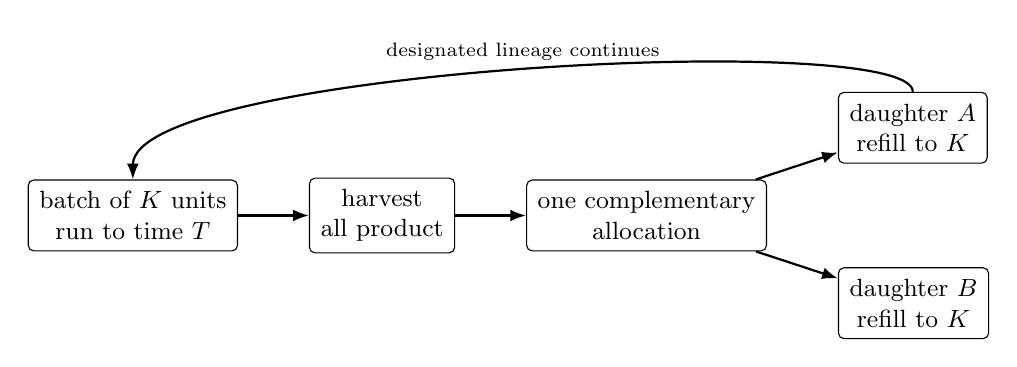
\begin{tikzpicture}[
  node distance=6mm and 9mm,
  box/.style={draw,rounded corners=2pt,align=center,inner sep=4pt,
              font=\small,minimum height=9mm},
  ar/.style={-{Latex[length=2mm]},thick}]
\node[box] (b) {batch of $K$ units\\ run to time $T$};
\node[box,right=of b] (h) {harvest\\ all product};
\node[box,right=of h] (s) {one complementary\\ allocation};
\node[box,above right=2mm and 9mm of s] (da) {daughter $A$\\ refill to $K$};
\node[box,below right=2mm and 9mm of s] (db) {daughter $B$\\ refill to $K$};
\draw[ar] (b) -- (h);
\draw[ar] (h) -- (s);
\draw[ar] (s) -- (da);
\draw[ar] (s) -- (db);
\draw[ar] (da.north) .. controls +(0,8mm) and +(0,14mm) .. node[above,font=\scriptsize]
      {designated lineage continues} (b.north);
\end{tikzpicture}
\caption{The protocol of Definition~\ref{def:protocol}. Success is the single
event ``quota met \emph{and} both daughters back in the restart set''. The
same picture serves both encodings; only the restart set and the return
payoff $s_\theta$ change.}
\label{fig:protocol}
\end{figure}

\section{Encoding-independent obstructions}\label{sec:obstructions}

Three bounds hold for every source in the framework. They are necessary
conditions, never sufficient: a permitted terminal allocation is not a proof
that initially product-free chemistry reaches it by the deadline.

\subsection{The carrier ceiling}

\begin{theorem}[Carrier ceiling, C]\label{thm:ceiling}
Suppose the memory is carried by $m$ species, each of which must be present in
both daughters, all carriers are unit-weight and allocated independently and
fairly, and a quota of $q$ product units is harvested from the same conserved
pool of $K$ units. If the joint success probability is at least $1-\delta$ for
some $0<\delta<1$, then
\begin{equation}\label{eq:ceiling}
K\ \ge\ q+m\left\lceil 1+\log_2(1/\delta)\right\rceil .
\end{equation}
\end{theorem}

\begin{proof}
On the quota event the terminal carrier counts $r_1,\dots,r_m$ satisfy
$\sum_j r_j\le K-q$, so $\min_j r_j\le\lfloor (K-q)/m\rfloor=:r$. Both
daughters contain a given species with $r$ copies with probability at most
$1-2^{1-r}$ (zero if $r=0$), and the joint event is contained in that one.
Averaging over terminal states preserves the inequality, so
$1-\delta\le1-2^{1-r}$, i.e.\ $2^{1-r}\le\delta$, i.e.\
$r\ge1+\log_2(1/\delta)$. Since $r$ is an integer,
$\lfloor(K-q)/m\rfloor\ge\lceil1+\log_2(1/\delta)\rceil$, which is
\eqref{eq:ceiling}. \leanref{\texttt{quota\_limits\_carriers},
\texttt{reliability\_requires\_carriers}, \texttt{material\_necessary}}
\end{proof}

At $q=4$ and $\delta=10^{-3}$ this excludes $K\le14$ for support memory
($m=1$; the relevant ceiling at $K=14$ is $511/512<999/1000$) and
$K\le25$ for two-type memory. The bound is a ceiling within the stated
intact-object partition architecture, not a universal law.

\subsection{Material cannot buy time}

\begin{theorem}[First-enabling obstruction, C]\label{thm:clock}
Let $z$ be an admitted restart state at which the total enabled exit rate is
$a(z)$, and suppose a positive quota requires at least one reaction to fire.
Then for every material budget,
\begin{equation}\label{eq:clock}
p_*\ \le\ 1-e^{-a(z)T}.
\end{equation}
Consequently a uniform target $1-\delta$ requires $a(z)\,T\ge\log(1/\delta)$
at every admitted restart state.
\end{theorem}

\begin{proof}
The first holding time at $z$ is exponential with rate $a(z)$, so with
probability $e^{-a(z)T}$ the chain has not moved by $T$ and the terminal
product is zero. \end{proof}

This is the sharpest structural statement in the paper, because it is
completely insensitive to $K$: no amount of added food removes it. For the
support-memory source of \S\ref{sec:support} the admitted bound seed
$(n,c,p,f)=(0,1,0,K-2)$ has exactly two enabled exits, each of rate $\kappa$,
whence $p_*\le1-e^{-2\kappa T}$; at $T=5$ and $\delta=10^{-3}$ every release
rate $\kappa<\log(1000)/10\simeq0.690776$ is infeasible at every budget.
\leanref{\texttt{bound\_seed\_admitted}, \texttt{bound\_seed\_rates}}

\begin{corollary}[Order and material are substitutes, C]\label{cor:order}
In stochastic mass action at fixed reference volume, a channel of molecularity
$r$ with rate constant $k$ has propensity at most $k\,K^{r}$ on a pool of $K$
units. Hence a uniform target $1-\delta$ requires
\begin{equation}\label{eq:order}
k\,K^{r}\,T\ \ge\ \log(1/\delta).
\end{equation}
\end{corollary}

Inequality \eqref{eq:order} is the quantitative form of the trade-off this
paper is about. A network that is denied large $k$ and large $r$ --- an
elementary network with physically bounded constants --- must buy its clock
with $K$. A formal network that is allowed unbounded $r$ and unbounded $k$
gets its clock for nothing, and then pays for something else. Sections
\ref{sec:support} and \ref{sec:proportion} are the two ends of that trade.

\subsection{Corridors must contain their own increment}

\begin{lemma}[Corridor necessity, C]\label{lem:corridor}
Consider a coordinate whose newborn count lies anywhere in $[l,u]$ and which
gains a fixed increment $g$ before division, so that the parent count ranges
over $[l+g,u+g]$, and suppose both daughters must return to $[l,u]$ with
positive probability uniformly over newborns. Then $l\le g\le u$.
\end{lemma}

\begin{proof}
From the newborn with count $l$ the parent holds $l+g$ objects and the
daughters receive $I$ and $l+g-I$; both are at least $l$ only if
$l\le I\le g$, an empty range when $g<l$. From the newborn with count $u$ the
parent holds $u+g$ and both daughters are at most $u$ only if $g\le I\le u$,
empty when $g>u$. \end{proof}

So a corridor memory must grow by an amount lying inside its own corridor.
Support memory has no analogue of this constraint, and
\S\ref{sec:proportion} shows it is what makes the difference in cost.

\section{Support memory at the elementary frontier}\label{sec:support}

\subsection{The source}

Fix the label $S\in\{X,Y\}$ and take the three reversible pairs
\begin{equation}\label{eq:supportsource}
S+F\rightleftharpoons 2S,\qquad
S+F\rightleftharpoons C_S,\qquad
C_S\rightleftharpoons S+P_S,
\end{equation}
with forward/reverse constants $(1,1/100)$, $(2,\kappa)$ and
$(\kappa,1/50)$. Only the selected label is initially present, and no channel
creates the other label, so its absence is invariant: this is
support-encoded memory, and contamination correction is outside the theorem.
Every reaction in \eqref{eq:supportsource} is at most bimolecular.

At fixed reference volume write $z=(n,c,p)$ for the counts of free carrier,
complex and product, with food reconstructed as $f=K-n-2c-p$. The state space
and restart set are
\begin{equation}
\Omega_K=\{n+2c+p\le K,\ n+c\ge1\},\qquad
\mathcal{B}_K=\{(n,c,0)\in\Omega_K:1\le n+c\le K-1\},
\end{equation}
and the six destination increments and propensities are
\begin{equation}\label{eq:channels}
\begin{array}{llll}
(+1,0,0)\ \ nf, &\quad (-1,0,0)\ \ n(n-1)/100, &\quad (-1,+1,0)\ \ 2nf,\\[2pt]
(+1,-1,0)\ \ \kappa c, &\quad (+1,-1,+1)\ \ \kappa c, &\quad
(-1,+1,-1)\ \ np/50 .
\end{array}
\end{equation}
Zero-rate channels are omitted; in particular there is no extra factor $1/2$
in reverse replication. A complex carries one carrier moiety and one
food-derived moiety, so the weighted material invariant is $n+2c+p+f=K$ while
the number of intact carrier-bearing partition objects is $R=n+c$. At $K=32$,
$|\Omega_{32}|=3\,384$ and $|\mathcal{B}_{32}|=287$.

\begin{remark}[No batch extinction]
Only reverse replication lowers $R$, and its propensity $n(n-1)/100$ vanishes
at $n\le1$; every other channel preserves $R$. The last carrier therefore
cannot disappear during a batch, and the relevant failures are exactly the two
in \eqref{eq:payoff}: missing the quota, or losing a daughter at the
allocation. \leanref{\texttt{jump\_conserves},
\texttt{final\_resident\_survives}}
\end{remark}

With payoff $h_q(z)=\one\{p\ge q\}(1-2^{1-(n+c)})$ define
\begin{equation}
p_*(K,\kappa)=\min_{z\in\mathcal{B}_K}(e^{5G_{K,\kappa}}h_4)(z),
\qquad
p_{\mathrm{rob}}(K)=\inf_{10\le\kappa\le20}p_*(K,\kappa).
\end{equation}
The generator acts on a column payoff; no transpose is used.

\subsection{The robust exact minimum}

\begin{theorem}[Robust exact minimum, C/E]\label{thm:min32}
The least integer $K\ge2$ with $p_{\mathrm{rob}}(K)\ge999/1000$ is exactly
$32$. In fact
\begin{equation}\label{eq:L}
p_{\mathrm{rob}}(32)\ \ge\ L:=\frac{2\,145\,514\,420}{2^{31}}
=0.999083006754\ldots
\end{equation}
Every $K\le14$ is excluded by Theorem~\ref{thm:ceiling} and every
$15\le K\le31$ by an exact upper certificate at the admitted constant
parameter $\kappa=10$, the largest being
$U_{31}=2\,144\,298\,834/2^{31}=0.998516955\ldots$ Consequently the same
minimum holds for every reliability target $\rho$ with
$U_{31}<\rho\le L$.
\end{theorem}

The proof occupies \S\S\ref{sec:envelope}--\ref{sec:integer}; the exclusion
table is Table~\ref{tab:nominal} and the whole computation is replayed by
\texttt{scripts/frontier\_support.py}. Three features deserve emphasis. The
statement is a \emph{robust} minimum: it does not say that every $K<32$ fails
at every release rate, only that no $K<32$ guarantees the target across the
whole band. No monotonicity in $K$, $T$ or $\kappa$ is used or proved --- the
finite list is checked budget by budget. And it is not asserted that every
$K>32$ succeeds.

\begin{remark}[Where the $17$ units go]
The ceiling \eqref{eq:ceiling} permits $K=15$; the source requires $32$. The
$17$-unit difference is the price of the kinetics --- the deadline, the rate
band, the breadth of the restart set, product variability, residual food and
complex occupancy together. It is not a measured ``sequestration cost'' and we
do not allocate it to any single mechanism. What we \emph{can} exclude is that
it is certificate slack: at $K=32$ the certified lower value falls about
$1.05\times10^{-5}$ below the floating worst-start value, whereas $K=31$ fails
by an exact \emph{upper} bound, so no sharpening of the lower-bound algorithm
could rescue it.
\end{remark}

\subsection{The endpoint-kernel envelope}\label{sec:envelope}

The band $[10,20]$ is a continuum, and the terminal probability is not known
to be monotone in $\kappa$. The certificate avoids both difficulties by
applying convexity to the one-step \emph{kernel} and never to a deadline
probability.

Choose an integer clock $\lambda$ at least as large as every exit rate across
the band. At $K=32$ the exit rate
$3nf+n(n-1)/100+2\kappa c+np/50$ is affine and increasing in $\kappa$, so it is
largest at $\kappa=20$, where its maximum over $\Omega_{32}$ is $770.4$,
attained at $(n,c,p)=(16,0,0)$ --- a state holding no complex, so the value is
the same at both endpoints. Hence $\lambda=771$ is valid throughout the band. Put $P_\kappa=I+G_\kappa/\lambda$. Each $P_\kappa$
is stochastic, and because the generator is affine in $\kappa$,
\begin{equation}\label{eq:affine}
P_\kappa=(1-t)P_{10}+tP_{20},\qquad t=(\kappa-10)/10\in[0,1].
\end{equation}
\leanref{\texttt{release\_affine}}

\begin{lemma}[Envelope, C; K]\label{lem:envelope}
Define the nonlinear operator $(Mv)(z)=\min\{(P_{10}v)(z),(P_{20}v)(z)\}$.
Then $M$ is monotone, $Mv\le P_\kappa v$ for every $\kappa$ in the band, and
$M^{j}v\le P_\kappa^{j}v$ for every $j\ge0$. For $v\ge0$ and every
$J\in\N$,
\begin{equation}\label{eq:poisson}
e^{-1}\sum_{j=0}^{J}\frac{M^{j}v}{j!}\ \le\
e^{-1}\sum_{j=0}^{\infty}\frac{P_\kappa^{j}v}{j!}=e^{G_\kappa/\lambda}v .
\end{equation}
\end{lemma}

\begin{proof}
Both $P_{10}$ and $P_{20}$ are nonnegative, so each is monotone and hence so
is their pointwise minimum. The scalar inequality
$\min(a,b)\le(1-t)a+tb$ for $t\in[0,1]$ together with \eqref{eq:affine} gives
$Mv\le P_\kappa v$ entrywise. The iterate bound follows by induction:
$M^{j+1}v=M(M^{j}v)\le M(P_\kappa^{j}v)\le P_\kappa(P_\kappa^{j}v)$, the first
step by monotonicity of $M$ and the second by the previous sentence. Finally
the omitted terms of the Poisson sum are nonnegative because $v\ge0$ and both
kernels are nonnegative. \leanref{\texttt{envelope\_le\_kernel},
\texttt{envelope\_iterates\_lower}, \texttt{envelope\_nonneg},
\texttt{robust\_poisson\_lower}}
\end{proof}

Composing $\lambda T$ such blocks preserves the lower bound for every fixed
$\kappa$ in the band, which is all Theorem~\ref{thm:min32} requires. The
rowwise minimum permits a different adverse endpoint at each state and each
iteration depth, so the certificate is in general \emph{conservative} relative
to any single fixed $\kappa$; we make no claim that it equals the
fixed-parameter infimum. What must not be done --- and is not done here --- is
to interchange minimisation with matrix exponentiation.

\begin{remark}[Reusable form]
Nothing above is specific to chemistry or to two endpoints. If a family of
generators lies in the convex hull of $G_1,\dots,G_m$ and one common clock is
valid for all of them, then $Mv=\min_i P_iv$ certifies every generator in the
hull. A parameter box entered affinely lies in the hull of its vertex
generators; nonlinear parameter dependence needs a separate enclosure. This is
how \S\ref{sec:enlarged} certifies a six-dimensional rate box.
\end{remark}

\begin{lemma}[Complement, C; K]\label{lem:complement}
Because the full stochastic semigroup preserves constants,
$e^{TG}h=1-e^{TG}(1-h)$. Hence a lower certificate $\ell$ for the payoff
$1-h$ yields the upper certificate $e^{TG}h\le1-\ell$.
\leanref{\texttt{complement\_upper}}
\end{lemma}

Lemma~\ref{lem:complement} is what makes the exclusions in
Theorem~\ref{thm:min32} genuine: a lower bound falling below the target proves
nothing, whereas an upper bound below the target at one admitted start
excludes the budget outright. One admitted witness suffices to exclude;
inclusion requires all $287$ starts.

\subsection{Exact integer implementation}\label{sec:integer}

Let $\Scale=2^{31}$, $D=100\lambda=77\,100$, and let $A_i=DP_i$ for the two
endpoints; every entry of $A_i$ is a nonnegative integer and every row sums to
$D$. Let
\begin{equation}
e_-=\sum_{j=0}^{25}\frac{(-1)^j}{j!}\ \in(0,e^{-1}),
\qquad w_j=\left\lfloor \Scale\,e_-/j!\right\rfloor\ (0\le j\le18),
\end{equation}
the alternating partial sum being a valid strict lower bound for $e^{-1}$
because it terminates on a negative term; integer weights vanish beyond
$j=12$. Starting from $v=\lfloor \Scale h\rfloor$, one block is
\begin{equation}\label{eq:block}
v_0=v,\qquad
v_{j+1}=\left\lfloor\frac{\min(A_{10}v_j,\,A_{20}v_j)}{D}\right\rfloor,
\qquad
\mathcal{B}v=\left\lfloor\frac{\sum_{j=0}^{18}w_jv_j}{\Scale}\right\rfloor,
\end{equation}
all floors and minima componentwise, repeated $\lambda T=3\,855$ times.

\begin{proposition}[Soundness and overflow safety, C]\label{prop:sound}
Every intermediate vector of \eqref{eq:block}, divided by $\Scale$, is a lower
bound for the corresponding quantity in \eqref{eq:poisson}; and the
computation cannot overflow signed \texttt{int64}.
\end{proposition}

\begin{proof}
Rounding is downward at every step and the omitted Poisson terms are
nonnegative, so both sources of error have the correct sign; the inductive
hypothesis $v_j/\Scale\le M^{j}(h)$ is preserved by
Lemma~\ref{lem:envelope} and the monotonicity of $x\mapsto\lfloor x\rfloor$.
For the bound, $0\le v_i\le \Scale$ throughout, so each sparse row product is
at most $D\Scale<2^{63}$ and the weighted accumulator at most
$\Scale\sum_j w_j\le \Scale^2<2^{63}$. The two payoff columns are carried
separately and never added. Threshold comparisons are exact integer
cross-products. \end{proof}

The stationary distribution, floating solvers and trajectory plots supply no
input to this certificate. \textbf{Trust boundary.} Exact integer arithmetic
removes rounding from the recurrence; it does not make the construction of
states, destinations, matrices and loops formally verified. That construction,
and the identification of the finite generator and its Poissonised semigroup
with the physical protocol, are conventional (\textbf{C}); see
\S\ref{sec:lean}.

\begin{table}[t]
\centering\small
\caption{Exact two-sided certificates at $\kappa=10$, $T=5$, $q=4$;
denominator $2^{31}=2\,147\,483\,648$ throughout. Every excluded row carries
the admitted upper witness $(K-1,0,0)$; the included row covers all $287$
starts. The largest excluded upper value is at $K=31$. Appendix~\ref{app:replay}
records an independent reimplementation that reproduces every entry.}
\label{tab:nominal}
\begin{tabular}{rrrr@{\qquad}rrrr}
\toprule
$K$ & states & lower & upper & $K$ & states & lower & upper\\
\midrule
15 & 428  & 1015891063 & 1015896977 & 24 & 1522 & 2072944721 & 2072959911\\
16 & 508  & 1220976456 & 1220983211 & 25 & 1703 & 2097931806 & 2097948254\\
17 & 597  & 1410294481 & 1410302076 & 26 & 1898 & 2115061624 & 2115079437\\
18 & 696  & 1576864428 & 1576872967 & 27 & 2107 & 2126576039 & 2126595217\\
19 & 805  & 1717234717 & 1717244202 & 28 & 2331 & 2134178444 & 2134199094\\
20 & 925  & 1831016096 & 1831026631 & 29 & 2570 & 2139116888 & 2139139042\\
21 & 1056 & 1920060288 & 1920071907 & 30 & 2825 & 2142277641 & 2142301368\\
22 & 1199 & 1987562186 & 1987574961 & 31 & 3096 & 2144273535 & 2144298834\\
23 & 1354 & 2037277175 & 2037291104 & \textbf{32} & \textbf{3384}
                                    & \textbf{2145518355} & \textbf{2145545336}\\
\bottomrule
\end{tabular}
\end{table}

The robust lower numerators at $K=32$ are $2\,145\,517\,682$ for the band
$[10,11]$ and $2\,145\,514\,420$ for $[10,20]$; only the second is needed. The
wider band costs just $3\,935$ integer units --- about
$1.83\times10^{-6}$ --- relative to the nominal lower certificate, so
certifying a factor-two rate band is nearly free here. The enclosure of the robust value is
\begin{equation}
\frac{2\,145\,514\,420}{2^{31}}\ \le\ p_{\mathrm{rob}}(32)\ \le\
\frac{2\,145\,545\,336}{2^{31}},
\end{equation}
of width about $1.44\times10^{-5}$, the upper bound coming from the admitted
value $\kappa=10$.

\subsection{Enlarged robustness: bias and a rate box}\label{sec:enlarged}

Two idealisations in Definition~\ref{def:protocol} invite attack: that the
allocation coin is exactly fair, and that the six rate constants are exactly
the declared rationals. Both can be removed without recomputing the model from
scratch, and the tolerances are far larger than a perturbative estimate
suggests.

\paragraph{Allocation bias.} Replace the fair coin by independent allocation
to daughter $A$ with a common probability $\theta$, the daughters still
complementary. The terminal payoff becomes $h_{q,\theta}=\one\{p\ge
q\}s_\theta(R)$ with $s_\theta$ as in \eqref{eq:sfair}. For fixed $R\ge1$ the
function $\theta\mapsto\theta^{R}+(1-\theta)^{R}$ is convex and symmetric
about $1/2$, so it is maximised over any interval $[\theta_0,1-\theta_0]$ at
the endpoints: certifying at $\theta_0$ certifies the whole interval. Running
the envelope certificate with that payoff --- rather than bounding the payoff
difference --- gives the following.

\begin{theorem}[Bias tolerance, C/E]\label{thm:bias}
For every $\theta\in[39/100,\,61/100]$ and every $\kappa\in[10,20]$, the
$K=32$ source meets the target:
\[
\min_{z\in\mathcal{B}_{32}}\Pr_z(\text{joint success})\ \ge\
\frac{2\,145\,366\,143}{2^{31}}=0.999063\ldots>\frac{999}{1000}.
\]
Because $\theta=1/2$ lies in the family, every $K<32$ remains excluded, so
$32$ is still the exact robust minimum over this enlarged uncertainty set. At
$\theta=19/50$ the guarantee genuinely fails: the exact upper certificate at
the admitted bound seed $(0,1,0)$ is $2\,145\,078\,112/2^{31}<999/1000$.
\end{theorem}

An $11$ percentage-point tolerance in the allocation bias is a substantive
robustness statement: it is $22$ times the $\pm0.005$ that a
payoff-perturbation argument charged against the margin, and it is obtained
at the same computational cost as the original certificate. Note also that the
worst admitted start migrates from the resident-heavy $(31,0,0)$ to the bound
seed $(0,1,0)$ as the bias grows, which is why a fixed-worst-start shortcut
would be unsound.

\paragraph{A simultaneous rate box.} Let each of the six rate constants in
\eqref{eq:supportsource} be perturbed independently by a factor in
$[1-\varepsilon,1+\varepsilon]$, the two complex-exit constants remaining tied
to one another and ranging over $[10(1-\varepsilon),20(1+\varepsilon)]$. The
generator is jointly affine in these five group parameters, so the family lies
in the convex hull of its $2^{5}$ vertex generators, and the envelope of
Lemma~\ref{lem:envelope} applies with $Mv=\min_i P_iv$ over the vertices ---
equivalently, groupwise, with the rowwise minimum computed one group at a
time.

\begin{theorem}[Rate-box tolerance, C/E]\label{thm:box}
At $\varepsilon=1/300$ the $K=32$ source meets the target uniformly over the
whole box and the whole release band, with exact lower certificate
$2\,145\,342\,442/2^{31}=0.999052\ldots$ (integer clock $773$). The exact
minimum is therefore still $32$ under simultaneous $\pm0.33\%$ uncertainty in
every rate constant.
\end{theorem}

Since multiplying all six constants by a common factor is a time rescaling,
Theorem~\ref{thm:box} also absorbs a $\pm0.33\%$ uncertainty in the deadline.
At $\varepsilon=1/250$ our lower certificate falls below the target while the
upper certificate stays above it, so that case is undetermined, not excluded;
we report it as such.

\subsection{A direction in which it breaks}\label{sec:branching}

Theorems~\ref{thm:bias} and \ref{thm:box} might suggest that the $32$-unit
result is robust in every direction. It is not, and the exception is
instructive.

In \eqref{eq:supportsource} the bound complex has two exits, $C_S\to S+F$ and
$C_S\to S+P_S$, and the source gives them the \emph{same} constant $\kappa$:
the complex is equally likely to dissociate as to release product. Let us
untie them, writing $\kappa_d$ for dissociation and $\kappa_r$ for release.
This changes no molecularity, adds no species and keeps the complex's total
lifetime under control; it changes only the branching ratio
$\kappa_r/(\kappa_d+\kappa_r)$.

\begin{theorem}[Branching frontier, C/E]\label{thm:min42}
At the fixed parameters $(\kappa_d,\kappa_r)=(20,10)$, with $T=5$, $q=4$ and
target $999/1000$, the budget $K=32$ is excluded by the exact upper
certificate $2\,104\,161\,482/2^{31}=0.979827\ldots$, and the least admissible
budget is exactly $42$, with exact lower certificate
$2\,145\,488\,787/2^{31}=0.999071\ldots$ Every $K\le14$ is excluded by
Theorem~\ref{thm:ceiling} and every $15\le K\le41$ by an exact upper
certificate at the admitted start $(K-1,0,0)$.
\end{theorem}

Halving the productive branching fraction therefore costs $10$ further
material units, a $31\%$ surcharge, without changing a single reaction. The
two frontiers are drawn together in Figure~\ref{fig:support}.

More surprisingly, the guarantee is not monotone in the product-release rate
either. At $(\kappa_d,\kappa_r)=(10,20)$ --- the complex now twice as likely
to make product as to fall apart --- the budget $K=32$ is again excluded, by
the exact upper certificate $2\,144\,643\,824/2^{31}=0.998678\ldots$ --- and
this time the excluding witness is the \emph{bound seed} $(0,1,0)$, not the
resident-heavy start. Raising only the productive channel breaks a
specification that the balanced source meets.

\paragraph{Why.} The dissociation channel is not futile. It returns the
food-derived moiety of the complex to the food pool, and food is the substrate
of $S+F\to2S$, the only channel that increases the carrier count $R$ on which
the partition payoff $1-2^{1-R}$ depends. The complex therefore arbitrates
between the two failure modes of \eqref{eq:payoff}, and the diagnostics in
Table~\ref{tab:branching} show both sides of the trade.

\begin{table}[t]
\centering\small
\caption{Terminal diagnostics at $K=32$, $T=5$, $q=4$, from the backward
equations solved in floating point (evidence \textbf{N}; no certificate uses
them). The balanced row is the reference decomposition
$9.00058131\times10^{-4}$ and $4.581103\times10^{-6}$. The worst admitted
start differs between settings, which is exactly why uniformity over the
restart set matters.}
\label{tab:branching}
\begin{tabular}{llrrrrr}
\toprule
$(\kappa_d,\kappa_r)$ & start & quota fail & partition fail &
$\E[R]$ & $\E[\text{food}]$ & $\E[p]$\\
\midrule
$(20,10)$ & $(31,0,0)$ & $2.017\times10^{-2}$ & $7.45\times10^{-7}$
          & 23.37 & 0.202 & 8.01\\
$(20,10)$ & $(0,1,0)$  & $1.469\times10^{-3}$ & $1.03\times10^{-5}$
          & 20.35 & 0.208 & 11.03\\[2pt]
$(10,10)$ & $(31,0,0)$ & $9.001\times10^{-4}$ & $4.58\times10^{-6}$
          & 20.73 & 0.154 & 10.61\\
$(10,10)$ & $(0,1,0)$  & $4.04\times10^{-6}$  & $1.865\times10^{-4}$
          & 15.99 & 0.155 & 15.39\\[2pt]
$(10,20)$ & $(31,0,0)$ & $1.74\times10^{-5}$  & $1.78\times10^{-5}$
          & 18.65 & 0.116 & 12.94\\
$(10,20)$ & $(0,1,0)$  & $1.70\times10^{-9}$  & $1.325\times10^{-3}$
          & 12.68 & 0.108 & 18.97\\
\bottomrule
\end{tabular}
\end{table}

Favouring dissociation raises the expected carrier count from $20.7$ to
$23.4$ and drives the expected harvest down from $10.6$ to $8.0$: the
resident-heavy start now misses its quota with probability $2\times10^{-2}$.
Favouring release does the opposite --- the quota failure at that start
collapses to $1.7\times10^{-5}$ --- but the food stock falls, the carrier
count at the seed-like starts falls from $16.0$ to $12.7$, and those starts
now lose a daughter with probability $1.3\times10^{-3}$. The balanced source
sits between two distinct failure modes, and the $0.999$ specification at
$K=32$ is available only in a window around it.

\begin{figure}[t]
\centering

\includegraphics{figures/support_frontier.pdf}
\caption{Exact two-sided certificates for the support-memory source. Plotted
is the certified upper bound on worst-start failure, i.e.\ $1-U_K$; the
budgets marked with stars are the exact minima, where the plotted value is the
certified lower bound's failure. Discrete certificates, not an interpolated
guarantee. Untying the complex's two exits at
$(\kappa_d,\kappa_r)=(20,10)$ shifts the frontier from $32$ to $42$.}
\label{fig:support}
\end{figure}

\section{Proportion memory with a cooperative gate}\label{sec:proportion}

\subsection{The architecture class}

Proportion memory keeps both species at all times, so the failure mode of
\S\ref{sec:support} --- a daughter with no carrier --- is replaced by the much
more demanding requirement that each daughter's counts re-enter a corridor.
No elementary network achieving this under a finite-count deadline guarantee
is known to us. The route that does work trades reaction order for exact
tractability, and we now define the whole class so that it can be optimised
rather than merely exhibited.

\begin{definition}[The class $\mathcal{G}(q)$]\label{def:class}
Fix integers $1\le l_Y\le u_Y<l_X\le u_X$, increments $g_X,g_Y\ge1$ and a
quota $q\ge1$. The species are $X,Y,F,H,W,P_X,P_Y$, each of unit material
weight. The two reversible pairs are
\begin{align}
l_XX+l_YY+(g_X+g_Y+q)F+H
&\rightleftharpoons (l_X+g_X)X+(l_Y+g_Y)Y+qP_X+W, \label{eq:gate}\\
l_XY+l_YX+(g_X+g_Y+q)F+H
&\rightleftharpoons (l_X+g_X)Y+(l_Y+g_Y)X+qP_Y+W, \notag
\end{align}
in the fixed-volume falling-factorial convention, with positive rational
constants $k$ (forward) and $b$ (reverse). The conserved pools are
$x+y+f+p_X+p_Y=N$ and $h+w=1$. Program $0$ has newborn set
\begin{equation}\label{eq:newborn}
\mathcal{B}_0=\{\,l_X\le x\le u_X,\ l_Y\le y\le u_Y,\ f=N-x-y,\ h=1,\
w=p_X=p_Y=0\,\},
\end{equation}
program $1$ exchanges $x$ and $y$, and the decoder is the sign of $x-y$.
The protocol is Definition~\ref{def:protocol} with $T=1$: run, harvest all
product, allocate every intact molecule by one fair complementary coin,
discard the inherited $H/W$ token, refill food to core $N$ and supply one
fresh $H$.
\end{definition}

We call the member
$(l_X,u_X,g_X;l_Y,u_Y,g_Y;q)=(65,195,121;8,64,30;4)$ the \emph{reference
construction} $\mathcal{R}$. Its core is $N=414$, its initial supply $415$
including the fuel token, and both of its reaction directions have
molecularity $229$.

\begin{lemma}[Minimal core mass, C]\label{lem:core}
A member of $\mathcal{G}(q)$ with the stated corridors requires core mass at
least
\begin{equation}\label{eq:core}
N\ \ge\ c_X+c_Y+q,\qquad c_X:=u_X+g_X,\quad c_Y:=u_Y+g_Y,
\end{equation}
and $N=c_X+c_Y+q$ is attainable.
\end{lemma}

\begin{proof}
The gate \eqref{eq:gate} consumes $g_X+g_Y+q$ food units, and must be enabled
at every newborn, in particular the food-poorest one $x=u_X$, $y=u_Y$, where
$f=N-u_X-u_Y$. Hence $N-u_X-u_Y\ge g_X+g_Y+q$. \end{proof}

\begin{lemma}[Exact two-state closure, C; K]\label{lem:closure}
For every $z\in\mathcal{B}_0$ the reachable class of the full CTMC is exactly
$\{z,z^{*}\}$ with
\[
z^{*}=(x+g_X,\ y+g_Y,\ f-(g_X+g_Y+q),\ 0,\ 1,\ q,\ 0).
\]
\end{lemma}

\begin{proof}
At $z$ the mirror forward channel needs $l_X$ copies of $Y$ and is disabled
because $y\le u_Y<l_X$; both reverse channels need a product that is absent.
The selected forward channel is enabled by \eqref{eq:newborn} and
Lemma~\ref{lem:core}, and its unique successor is $z^{*}$. At $z^{*}$ both
forward channels are disabled because $h=0$, and the mirror reverse needs
$P_Y$, which is absent; the selected reverse is enabled and returns exactly to
$z$. These are all four channels of the source, so the class is closed. The
mirror program is the image under the label permutation. Distinct newborns
give distinct classes because subtracting the fixed increment recovers the
newborn. \leanref{\texttt{newborn\_only\_forward},
\texttt{grown\_only\_reverse}, \texttt{forward\_result},
\texttt{reverse\_result}, \texttt{exact\_closed\_pair}}
\end{proof}

This is an exact restriction of the literal chain, not an averaged projection
or a quasi-steady-state elimination, and it is what makes the class exactly
optimisable: the terminal law is a two-state law, and the entire finite-count
difficulty moves to the allocation stage.

\subsection{The clock is free; the corridor is not}

\begin{lemma}[Clock, C]\label{lem:clock}
Let $a$ be the forward rate at a newborn and $d$ the reverse rate at $z^*$.
The probability of occupying $z^{*}$ at time $T$ is exactly
\begin{equation}\label{eq:twostate}
r(a,d)=\frac{a}{a+d}\bigl(1-e^{-(a+d)T}\bigr).
\end{equation}
If $a\ge A$ and $d\le D$ then $r(a,d)\ge\frac{A}{A+D}(1-e^{-AT})$. Moreover
for any $A,D>0$ the choices
\begin{equation}\label{eq:constants}
k=\frac{A}{l_X!\,l_Y!\,(g_X+g_Y+q)!},\qquad
b=\frac{D}{(c_X)_{l_X+g_X}\,(c_Y)_{l_Y+g_Y}\,q!}
\end{equation}
achieve those bounds uniformly over the newborn set, where
$(n)_r=n!/(n-r)!$.
\end{lemma}

\begin{proof}
Equation \eqref{eq:twostate} solves $\dot\pi=a-(a+d)\pi$, $\pi(0)=0$. Both
factors are monotone in the stated directions. For \eqref{eq:constants}, the
forward propensity is $k\,(x)_{l_X}(y)_{l_Y}(f)_{g_X+g_Y+q}h$ and
$(n)_r\ge r!$ whenever $n\ge r$, which holds on the newborn set; the reverse
propensity is $b\,(x')_{l_X+g_X}(y')_{l_Y+g_Y}(p_X)_{q}w$ and each falling
factorial is maximised at the largest admitted count, namely $c_X$ and $c_Y$.
\leanref{\texttt{forward\_rate\_lower}, \texttt{reverse\_rate\_upper}}
\end{proof}

Because $k$ and $b$ are free positive rationals, $r(a,d)$ can be pushed
arbitrarily close to $1$ at no material cost. \emph{The clock in
$\mathcal{G}(q)$ is free.} By Lemma~\ref{lem:closure} the joint success
probability from a newborn $z$ is exactly
\begin{equation}\label{eq:jointprop}
\Pr_z(\text{success})=r(a,d)\cdot
\psi(x+g_X;l_X,u_X)\,\psi(y+g_Y;l_Y,u_Y),
\end{equation}
the product over the disjoint $X$- and $Y$-allocation objects conditional on
the terminal state $z^{*}$. Consequently the frontier of $\mathcal{G}(q)$ is
determined by the partition stage alone, and any kinetic constraint can only
raise it.

\subsection{The endpoint reduction}

Define, for a coordinate with corridor $[l,u]$ and increment $g$,
\begin{equation}\label{eq:Phi}
\Phi(l,u,g)=\min_{l+g\le n\le u+g}\psi(n;l,u),
\end{equation}
the uniform two-daughter return probability over all newborns of that
coordinate. A naive evaluation of \eqref{eq:Phi} for $\mathcal{R}$ visits $7\,467$ newborns per program. It is unnecessary.

\begin{lemma}[Endpoint reduction, C]\label{lem:endpoint}
Fix $l\le u$. The map $n\mapsto\psi(n;l,u)$ is nondecreasing for $n\le l+u$
and nonincreasing for $n\ge l+u$. Consequently the minimum in \eqref{eq:Phi}
is attained at an endpoint, and if $l\le g\le u$,
\begin{equation}\label{eq:closedforms}
\psi(l+g;l,u)=1-2\Pr\{\Bin(l+g,\tfrac12)\le l-1\},\qquad
\psi(u+g;l,u)=1-2\Pr\{\Bin(u+g,\tfrac12)\le g-1\}.
\end{equation}
Moreover $\psi(l+g;l,u)$ is nondecreasing in $g$ and nonincreasing in $l$,
and $\psi(u+g;l,u)$ is nonincreasing in $g$ at fixed $u+g$.
\end{lemma}

\begin{proof}
For $n\le l+u$ the constraint $I\ge l$ forces $n-I\le n-l\le u$, so the event
is exactly ``both daughters receive at least $l$''; for $n\ge l+u$ the
constraint $I\le u$ forces $n-I\ge n-u\ge l$, so it is exactly ``both
daughters receive at most $u$''. Couple the binomial counts as partial sums of
one Bernoulli sequence, so that $\Bin(n+1,\frac12)\ge\Bin(n,\frac12)$
pointwise. The first event is increasing in both daughter counts and the
second decreasing, which gives the two monotonicity statements and hence the
unimodality. For \eqref{eq:closedforms}: at $n=l+g$ the failure is
$\{I\le l-1\}\cup\{I\ge g+1\}$, two disjoint events of equal probability by
the symmetry $I\leftrightarrow n-I$; at $n=u+g$ the failure is
$\{I\ge u+1\}\cup\{I\le g-1\}$, likewise. For the last sentence, raising $g$
by one at fixed $l$ raises $n$ by one and leaves the threshold $l-1$ fixed,
and $\Pr\{\Bin(n+1)\le l-1\}\le\Pr\{\Bin(n)\le l-1\}$ by the same coupling;
raising $l$ by one raises both $n$ and the threshold by one, and
$\{\Bin(n)\le l-1\}\subseteq\{\Bin(n+1)\le l\}$. Raising $g$ at fixed $u+g$
raises the threshold $g-1$ alone. \end{proof}

So four binomial evaluations replace the whole table, and the search over
corridors becomes a two-parameter unimodal problem per coordinate. For $\mathcal{R}$, Lemma~\ref{lem:endpoint} gives the exact minimum
\begin{equation}\label{eq:Phistar}
\Phi_*=\Phi(65,195,121)\cdot\Phi(8,64,30)=0.999712941541084\ldots,
\end{equation}
attained at the newborn $(65,64)$ with productive parent $(186,94)$; the exact
rational value has an $84$-digit numerator and is recorded in
\texttt{data/frontier\_proportion.json}. A union bound over the four
endpoint tails gives instead $1-E$ with $E=4.25767634587\times10^{-4}$, hence
only the weaker constant $99957/100000$. The exact minimum recovers
$1.387\times10^{-4}$ of certificate slack, which was conservatism and not a
physical loss.
\leanref{\texttt{complementary\_binomial\_law},
\texttt{endpoint\_tail\_certificate}}

\subsection{Sharpened constants for $\mathcal{R}$}

Combining \eqref{eq:Phistar} with Lemma~\ref{lem:clock} at $A=20$,
$D=10^{-5}$, $T=1$ --- the rate bounds of $\mathcal{R}$ --- and
bounding $e^{20}$ below by its positive $25$-term Taylor sum, which exceeds
$4\times10^{8}$, gives
\begin{equation}\label{eq:rstar}
r_*=\frac{20}{20+10^{-5}}\Bigl(1-\frac{1}{4\times10^{8}}\Bigr)
=0.999999497500251\ldots
\end{equation}
and hence the following improvement.

\begin{theorem}[Sharpened guarantee, C/E]\label{thm:sharp}
For $\mathcal{R}$, uniformly over all $7\,467$
newborns of each program,
\[
\Pr(\text{joint success})\ \ge\ r_*\Phi_*=0.999712439185582\ldots\ >\
\frac{9997}{10000},
\]
and ten inspected cycles along a prescribed lineage succeed
jointly with probability at least $(9997/10000)^{10}>0.997$, collecting
forty fresh selected products.
\end{theorem}

The union-bound constants were $0.9995$ per cycle and $0.995$ over
ten; the guaranteed failure budget is thus more than halved, with no change to
the source, the protocol, the material account or the output. The
improvement is entirely a matter of replacing a union bound by the exact
endpoint minimum. We stress what is \emph{not} claimed: $r_*\Phi_*$ is a
product of the worst clock factor and the worst allocation factor, which need
not occur at the same newborn, so it is a valid lower bound and not the exact
minimum of the joint probability. The allocation minimum $\Phi_*$ is exact.

\begin{theorem}[Bias tolerance, C/E]\label{thm:biasprop}
$\mathcal{R}$ tolerates independent allocation bias $\theta\in[0.49,0.51]$:
the uniform partition probability is at least $0.999614114647\ldots$ and the
joint guarantee at least $r_*\cdot0.999614\ldots=0.999613612341\ldots>0.9996$.
At $\theta=0.48$ the uniform partition value drops to
$0.999220794519\ldots$ and the $0.9996$ guarantee is lost.
\end{theorem}

For fixed $\theta$ the accepted interval in \eqref{eq:psi} is
$[b,n-b]$ with $b=\max(l,n-u)$, which is symmetric about $n/2$; its binomial
mass is symmetric in $\theta\leftrightarrow1-\theta$ and increases as $\theta$
approaches $1/2$, because
$\frac{d}{d\theta}\Pr_\theta\{b\le I\le n-b\}
=n[\Pr_\theta\{J=b-1\}-\Pr_\theta\{J=n-b\}]$ with $J\sim\Bin(n-1,\theta)$,
whose bracket is nonnegative for $\theta\le1/2$ since the two binomial
coefficients agree. The parent-count reduction of Lemma~\ref{lem:endpoint}
holds for every fixed $\theta$, because its coupling argument never used
fairness. So interval endpoints in $\theta$ and parent-count endpoints in $n$
together reduce the claim to eight exact rational evaluations.

The bias window here, $\pm1$ percentage point, is an order of magnitude
narrower than the $\pm11$ points of Theorem~\ref{thm:bias}. This is the first
sign of the structural difference: a corridor is a two-sided constraint, and
a biased coin moves the daughter counts off centre in a way that presence
memory simply does not notice.

\subsection{The exact frontier}

We can now answer the question the construction leaves open.

\begin{theorem}[Frontier of $\mathcal{G}(q)$, C/E]\label{thm:frontier}
Let $q=4$ and let $\rho<1$ be a target.
\begin{enumerate}\itemsep2pt
\item[(i)] At $\rho=1999/2000$ --- specification of $\mathcal{R}$ --- the least core mass admitted by any member of
$\mathcal{G}(4)$ is $N=253$, attained by
$(l_X,u_X,g_X;l_Y,u_Y,g_Y)=(37,126,75;1,36,12)$ with exact uniform partition
probability $0.999529184472\ldots$ and reaction molecularity $130$.
\item[(ii)] If in addition every daughter is required to retain at least eight
minority molecules ($l_Y\ge8$, as $\mathcal{R}$ does), the least
core mass is $N=375$, attained by $(62,172,110;8,61,28)$, molecularity $213$.
\item[(iii)] At $\rho=999/1000$ --- the support-memory specification of
Theorem~\ref{thm:min32} --- the least core mass is $N=230$, attained by
$(33,115,68;1,32,11)$ with exact uniform partition probability
$0.999033665776\ldots$ and molecularity $118$.
\end{enumerate}
In each case the value is a minimum over the entire class, for every choice of
positive rational rate constants and every deadline.
\end{theorem}

\begin{proof}
By Lemma~\ref{lem:clock} the clock factor can be made to exceed any
$\rho'<1$, so a core mass $N$ is admissible if and only if some corridor
choice with $c_X+c_Y+q\le N$ has $\Phi_X\Phi_Y>\rho$; by Lemma~\ref{lem:core}
the cost is exactly $c_X+c_Y+q$. By Lemma~\ref{lem:corridor} we may restrict
to $l\le g\le u$, so $g\le c/2$ per coordinate, and by
Lemma~\ref{lem:endpoint} each $\Phi$ is the minimum of the two closed forms in
\eqref{eq:closedforms}. The monotonicity statements of
Lemma~\ref{lem:endpoint} show that at fixed $(g,c)$ the value is nonincreasing
in $l$, so the minority takes $l_Y$ at its declared floor and the majority
takes $l_X=u_Y+1$, the smallest value compatible with $u_Y<l_X$.

The search is therefore over $(c_Y,g_Y,c_X,g_X)$ and is exhaustive by the
following stopping rules, both of which are sound. First, since $\Phi_X\le1$,
any admissible pair has $\Phi_Y>\rho$, so minority candidates failing that are
discarded. Second, for each minority candidate the majority cost is scanned
upward from its minimum $2l_X$ and the first success is taken, which is the
true minimum for that candidate; and the enumeration of minority costs stops
as soon as $c_Y+q$ reaches the incumbent total, which is valid because
$c_X\ge2$. All arithmetic is exact rational. The witnesses and the
exhaustiveness are replayed by \texttt{scripts/frontier\_proportion.py}.
\end{proof}

Three readings of Theorem~\ref{thm:frontier}. First, $415$ was a construction,
not a cost: at its own specification the class does the job with $254$
supplied units, a $39\%$ saving, and with reaction order $130$ rather than
$229$. Second, most of the remaining gap to $\mathcal{R}$ is explained
by an undeclared constraint --- the requirement that each daughter keep at
least eight minority molecules, which is a stronger memory than the ratio
decoder needs. Making that constraint explicit raises the frontier to $375$,
much closer to $414$. Third, and this is the point of the merged comparison,
even the unconstrained frontier is an order of magnitude above the
support-memory minimum.

\subsection{Reliability scaling and the corridor cascade}\label{sec:scaling}

\begin{theorem}[Order of the frontier, C]\label{thm:order}
For $q\ge1$ and $\delta\in(0,1/2)$ let $N(\delta,q)$ denote the frontier of
$\mathcal{G}(q)$ at target $1-\delta$ with $l_Y\ge1$. Then
\begin{equation}\label{eq:order2}
q+2\log_2(2/\delta)\ \le\ N(\delta,q)\ \le\ q+20(z+2)^2+6,
\qquad z:=\sqrt{2\ln(8/\delta)},
\end{equation}
so $N(\delta,q)=q+\Theta(\log(1/\delta))$.
\end{theorem}

\begin{proof}
\emph{Lower bound.} At the minority newborn $y=l_Y$ the parent holds
$n_Y=l_Y+g_Y$ minority objects, and the failure event contains the two
disjoint all-to-one-daughter events, of total probability $2\cdot2^{-n_Y}$.
Hence $2^{1-n_Y}\le\delta$, i.e.\ $n_Y\ge\log_2(2/\delta)$. By
Lemma~\ref{lem:corridor}, $l_Y\le g_Y$, so $g_Y\ge n_Y/2\ge
\frac12\log_2(2/\delta)$. Again by Lemma~\ref{lem:corridor},
$u_Y\ge g_Y$, and by Definition~\ref{def:class} $l_X>u_Y\ge g_Y$, whence
$g_X\ge l_X>g_Y$ and $u_X\ge g_X>g_Y$. Therefore
$N=q+u_X+g_X+u_Y+g_Y\ge q+4g_Y\ge q+2\log_2(2/\delta)$.

\emph{Upper bound.} By Hoeffding's inequality \cite{hoeffding1963}
$\Pr\{|\Bin(n,\frac12)-n/2|\ge t\}\le2e^{-2t^{2}/n}$, so the failure of a
constraint of half-width $w/2$ at parent count $n$ is at most $\delta/4$ as
soon as $w\ge z\sqrt{n}$. Put $s=(z+2)^{2}$ and take
\[
l_Y=1,\quad g_Y=\lceil s\rceil,\quad u_Y=\lceil3s\rceil,\quad
l_X=u_Y+1,\quad g_X=\lceil6s\rceil+1,\quad u_X=\lceil10s\rceil+1 .
\]
Writing $\sqrt{s}=z+2$ and using $\sqrt{\alpha s+\beta}\le
\sqrt{\alpha}\,\sqrt s+\beta/(2\sqrt{\alpha s})$, each of the four conditions
$w\ge z\sqrt{n}$ reduces to a polynomial inequality in $z$ that holds for all
$z\ge1$: for the minority lower constraint $s-1\ge z\sqrt{s+2}$ since
$z^{2}+4z+3\ge z^{2}+2z+1$; for the minority upper constraint
$2s-1\ge z\sqrt{4s+2}$ since $2z^{2}+8z+7\ge2z^{2}+4z+1$; for the majority
lower constraint $3s-1\ge z\sqrt{9s+4}$ since $3z^{2}+12z+11\ge3z^{2}+7z$;
and for the majority upper constraint $4s-1\ge z\sqrt{16s+4}$ since
$4z^{2}+16z+15\ge4z^{2}+9z$. A union bound over the four gives success at
least $1-\delta$, and $z\ge1$ holds for every $\delta<1/2$. The core mass is
$N=q+u_X+g_X+u_Y+g_Y\le q+20s+6$. \end{proof}

The two constants in \eqref{eq:order2} are far apart, and the exact frontier
lies between them in a strikingly regular way. Table~\ref{tab:scaling} lists
it over five decades.

\begin{table}[t]
\centering\small
\caption{The exact frontier of $\mathcal{G}(4)$ with $l_Y\ge1$, over five
decades of target failure. The last column is $N/\ln(1/\delta)$; the
penultimate is the cascade prediction $20z_\delta^{2}$ with $z_\delta$ the
standard normal upper quantile at level $\delta$.}
\label{tab:scaling}
\begin{tabular}{lrlrrr}
\toprule
$\delta$ & $N$ & optimal corridors & molecularity &
$20z_\delta^{2}$ & $N/\ln(1/\delta)$\\
\midrule
$10^{-2}$ & 154 & $X[21,78]{+}45$, $Y[1,20]{+}7$    & 79  & 108 & 33.44\\
$10^{-3}$ & 230 & $X[33,115]{+}68$, $Y[1,32]{+}11$  & 118 & 191 & 33.30\\
$10^{-4}$ & 305 & $X[43,155]{+}90$, $Y[1,42]{+}14$  & 153 & 277 & 33.12\\
$10^{-5}$ & 384 & $X[54,196]{+}114$, $Y[1,53]{+}17$ & 191 & 364 & 33.35\\
$10^{-6}$ & 460 & $X[67,232]{+}137$, $Y[1,66]{+}21$ & 231 & 452 & 33.30\\
$10^{-7}$ & 537 & $X[77,273]{+}160$, $Y[1,76]{+}24$ & 267 & 541 & 33.32\\
\bottomrule
\end{tabular}
\end{table}

The ratio $N/\ln(1/\delta)$ is constant to within $1\%$ across the whole
range, so empirically $N\approx33.3\ln(1/\delta)$; we report this as an
observation about the computed values, not as a theorem. Its structure,
however, can be explained, and the explanation generalises.

\paragraph{The cascade.} Suppose all four constraints are tuned to the same
Gaussian margin, i.e.\ each corridor half-width equals $z$ standard deviations
of its binomial. Writing $l=\lambda z^{2}$, $g=\gamma z^{2}$, $u=\mu z^{2}$,
the two conditions per coordinate become
$\gamma-\lambda=\sqrt{\lambda+\gamma}$ and $\mu-\gamma=\sqrt{\gamma+\mu}$, and
the level-stacking constraint is $\lambda_{k+1}=\mu_k$. The unique solution
starting from $\lambda_1=0$ is given by the triangular numbers
$T_j=j(j+1)/2$:
\begin{equation}\label{eq:cascade}
l_k=T_{2k-2}z^{2},\qquad g_k=T_{2k-1}z^{2},\qquad u_k=T_{2k}z^{2},
\end{equation}
because $T_{2k-1}-T_{2k-2}=2k-1=\sqrt{T_{2k-2}+T_{2k-1}}$ and
$T_{2k}-T_{2k-1}=2k=\sqrt{T_{2k-1}+T_{2k}}$ --- both identities exact. The
$k$-th level therefore costs $c_k=(T_{2k}+T_{2k-1})z^{2}=4k^{2}z^{2}$, and $m$
ordered levels cost
\begin{equation}\label{eq:cubic}
N\ \approx\ q+z^{2}\sum_{k=1}^{m}4k^{2}
=q+\tfrac23\,m(m+1)(2m+1)\,z^{2}.
\end{equation}
For $m=2$ this is $20z^{2}$, the penultimate column of
Table~\ref{tab:scaling}; it agrees with the exact frontier to within $1.8\%$
at $\delta=10^{-6}$ and $0.7\%$ at $\delta=10^{-7}$, the residual at larger
$\delta$ coming from the minority's lowest constraint, which is a presence
bound rather than a corridor bound and is therefore cheaper than the Gaussian
balance assumes.

Equation \eqref{eq:cubic} predicts that reading an ordered $m$-level
composition costs $\Theta(m^{3}\log(1/\delta))$ material --- cubically more
than a single bit, because each level must clear the level below it,
and clearing a corridor of size $c$ costs $\Theta(\sqrt{c})$ of extra width
which then has to be re-grown. Table~\ref{tab:cascade} tests this against
exact computation with an equal per-level failure budget (a sufficient design,
so each entry is an exact upper bound on the $m$-level frontier; at $m=2$ it
reproduces the true frontier to within $1.5\%$). The per-level costs track
$k^{2}$ closely, and the agreement improves as $\delta$ decreases, as the
derivation requires.

\begin{table}[t]
\centering\small
\caption{Per-level corridor costs $c_k=u_k+g_k$ from exact computation with an
equal per-level budget $\delta/m$, normalised to the second level so that the
prediction $c_k\propto k^{2}$ reads $0.25:1:2.25:4$. The first level is
presence-limited rather than corridor-limited and is the outlier the cascade
derivation predicts.}
\label{tab:cascade}
\begin{tabular}{lrrrrl}
\toprule
$\delta$ & $c_1$ & $c_2$ & $c_3$ & $c_4$ & $c_k/c_2$\\
\midrule
$10^{-3}$ & 48 & 201 & 462 & 829 & $0.24:1:2.30:4.12$\\
$10^{-5}$ & 78 & 328 & 754 & 1359 & $0.24:1:2.30:4.14$\\
$10^{-7}$ & 108 & 458 & 1056 & 1902 & $0.24:1:2.31:4.15$\\
\midrule
prediction & --- & --- & --- & --- & $0.25:1:2.25:4$\\
\bottomrule
\end{tabular}
\end{table}

\subsection{The price of the gate}

The frontier is cheap in material only because the gate is expensive in
mechanism. The member of $\mathcal{G}(q)$ with parameters
$(l_X,u_X,g_X;l_Y,u_Y,g_Y;q)$ has reaction molecularity
\begin{equation}\label{eq:molecularity}
l_X+l_Y+(g_X+g_Y+q)+1
\end{equation}
in each direction --- $229$ for $\mathcal{R}$ and $130$ at the frontier of
Theorem~\ref{thm:frontier}(i). Along the frontier the cascade
\eqref{eq:cascade} makes it $(T_2+T_3+1)z^{2}=10z^{2}$ against a core of
$20z^{2}$, so molecularity is almost exactly $N/2$: it is
$79,118,153,191,231,267$ down the six rows of Table~\ref{tab:scaling}, and is
therefore $\Theta(\log(1/\delta))$ as well. Moreover the forward
propensity varies enormously over the newborn domain. For $\mathcal{R}$, $\log_{10}$ of the propensity ranges from $63.63$ at the vertex
$(195,64)$ to $121.87$ at $(118,14)$, a span of $10^{58.23}$; at the
$N=253$ frontier point the span is $10^{40.01}$. The minimum is at a vertex
for a reason: $\log$ of a product of falling factorials in $x$, $y$ and
$f=N-x-y$ is a sum of logarithms of positive affine functions, hence concave
on the newborn rectangle, and a concave function attains its minimum over a
polytope at a vertex. No rescaling removes this span, because multiplying all
forward constants by a positive scalar, or changing the global time unit,
preserves every dimensionless ratio.

So the material saving of \eqref{eq:cubic} conceals a mechanistic bill, and
Corollary~\ref{cor:order} says where it is paid. This is the honest reading of
the proportion-memory result: the class is a mathematical existence witness
with an exactly known material frontier, not a proposal for practical
chemistry. Replacing a $229$-body event by a chain of bimolecular reactions is
a separate substantive problem --- it changes intermediate stock,
sequestration, reaction races, leakage into the wrong program, the deadline
distribution and the partition --- and a coarse success bound $p$ transfers to
a refinement only as $p-\epsilon$, with $\epsilon$ a total-variation error
over a full cycle including the reset map, and with the intermediates' own
inventory charged.

\begin{figure}[t]
\centering

\includegraphics{figures/proportion_frontier.pdf}
\caption{The exact material frontier of the cooperative-gate class
$\mathcal{G}(4)$ against target reliability, with the cascade prediction
$20z_\delta^{2}$ of \eqref{eq:cubic}. $\mathcal{R}$
sits well above the frontier at its own specification.}
\label{fig:proportion}
\end{figure}

\section{Reading the two frontiers together}\label{sec:compare}

\begin{table}[t]
\centering\small
\caption{The two encodings at one specification: quota $q=4$, target
$0.999$, uniformity over the whole restart set, one complementary fair
allocation, refill to the working inventory, no post-division repair.}
\label{tab:compare}
\begin{tabular}{lll}
\toprule
& support memory & proportion memory\\
\midrule
stored object & which species is present & which species is in the majority\\
decoder & presence test & $x/(x+y)>1/2$\\
daughter must receive & at least one carrier & a count inside a corridor\\
kinetics & elementary, at most bimolecular & cooperative gate, order $118$\\
rate constants & fixed band $\kappa\in[10,20]$ & free positive rationals\\
deadline & $T=5$, fixed & free\\
carrier ceiling \eqref{eq:ceiling} & $15$ & $26$\\
\textbf{exact minimum material} & \textbf{32} & \textbf{231}\\
status of that number & minimum for this source & minimum over the whole class\\
allocation-bias tolerance & $\theta\in[0.39,0.61]$ & $\theta\in[0.49,0.51]$\\
scaling in $\log(1/\delta)$ & --- & $\approx33.3\ln(1/\delta)$\\
\bottomrule
\end{tabular}
\end{table}

Table~\ref{tab:compare} is the merged result. Four remarks on how to read it.

\paragraph{The comparison is conservative against proportion memory only in
one direction, and it is the direction that matters.} The number $32$ is the
minimum \emph{for one specific elementary network} at a fixed rate band and a
fixed deadline; some other elementary support-memory network might do better,
so $32$ is an upper bound on the true cost of support memory under those
constraints. The number $231$ is a minimum over an entire class in which
reaction order, rate constants and deadline are all free; every member of that
class pays at least that much. So the gap of roughly a factor of seven is a
lower bound on the gap, not an artefact of comparing a good design with a bad
one.

\paragraph{The extra cost is the corridor, not the clock and not presence.}
The carrier ceiling \eqref{eq:ceiling} charges proportion memory only $26$
units, against $15$ for support memory: keeping both species \emph{present}
is nearly free. Lemma~\ref{lem:clock} shows the clock is free in
$\mathcal{G}(q)$ outright. What costs $204$ further units is
Lemma~\ref{lem:corridor} and its consequences: a count must land inside a
window, the window must be wide enough to absorb binomial fluctuation of order
$\sqrt{N}$, and the growth increment that re-centres it must itself lie inside
the window. That is the whole of the difference, and \eqref{eq:cubic} is its
asymptotic form.

\paragraph{The two encodings fail differently under a biased coin.} Support
memory tolerates $\theta\in[0.39,0.61]$ and proportion memory only
$[0.49,0.51]$, a twentyfold difference in tolerance, for the same structural
reason: a presence constraint is one-sided and a corridor is two-sided.

\paragraph{Neither frontier is monotone in what it looks like it should be
monotone in.} Section~\ref{sec:branching} shows that the support-memory
frontier moves the wrong way when the productive channel is made faster,
because the apparently futile dissociation channel is what recycles the food
that builds carriers. Theorem~\ref{thm:frontier}(ii) shows that demanding
\emph{more} of the memory --- eight minority molecules rather than one ---
costs $122$ further units, so ``retain both species'' and ``retain eight
copies of each'' are quantitatively different specifications. In both cases
the lesson is the same: these systems have two competing failure modes on one
probability law, and intuitions calibrated on either mode alone mislead.

\section{Formal verification boundary}\label{sec:lean}

The developments compile in Lean~4 \cite{demoura2021} (toolchain
\texttt{leanprover/lean4:v4.30.0}) against a frozen Mathlib
\cite{mathlib2020}, under strict receipts: exit code
zero, warnings as errors, and an axiom report for each exported declaration.
All exported declarations depend only on \texttt{propext},
\texttt{Classical.choice} and \texttt{Quot.sound}; no \texttt{sorry} and no
numerical-answer axiom is present, and the exact tail certificate uses
ordinary \texttt{decide} with kernel reduction, not \texttt{native\_decide}.
Receipts are in \texttt{companion/verification/}.

\begin{table}[t]
\centering\small
\caption{Declaration map. Namespace \texttt{UsefulChemicalMemoryCost} (support
memory) and \texttt{ProductiveChemicalHeredity} (proportion memory).}
\label{tab:lean}
\begin{tabular}{>{\raggedright\arraybackslash}p{0.42\textwidth}>{\raggedright\arraybackslash}p{0.50\textwidth}}
\toprule
statement & declaration\\
\midrule
material conservation and survival of the last carrier &
\texttt{jump\_conserves}, \texttt{final\_resident\_survives}\\
quota charges material; carrier necessity; Theorem~\ref{thm:ceiling} &
\texttt{quota\_limits\_carriers}, \texttt{reliability\_requires\_carriers},
\texttt{material\_necessary}\\
generator affine in the release parameter &
\texttt{release\_affine}\\
bound seed admitted, with only its two exits &
\texttt{bound\_seed\_admitted}, \texttt{bound\_seed\_rates}\\
Lemma~\ref{lem:envelope} (envelope, iterates, Poisson block) &
\texttt{envelope\_le\_kernel}, \texttt{envelope\_iterates\_lower},
\texttt{envelope\_nonneg}, \texttt{robust\_poisson\_lower}\\
Lemma~\ref{lem:complement} (complement) & \texttt{complement\_upper}\\
complementary daughters return; refill identity &
\texttt{complementary\_daughter\_return}, \texttt{actual\_refill\_account}\\
exact margins around $L$, $U_{31}$ and $511/512$; ten-cycle margin &
\texttt{exact\_frontier\_margins}, \texttt{ten\_cycle\_margin},
\texttt{publication\_arithmetic}\\
exclusion from one admitted witness; minimum from finite coverage &
\texttt{robust\_exclusion}, \texttt{exact\_minimum\_from\_coverage}\\
\midrule
Lemma~\ref{lem:closure} (two-state closure) &
\texttt{newborn\_only\_forward}, \texttt{grown\_only\_reverse},
\texttt{forward\_result}, \texttt{reverse\_result},
\texttt{exact\_closed\_pair}\\
Lemma~\ref{lem:clock} rate bounds &
\texttt{forward\_rate\_lower}, \texttt{reverse\_rate\_upper}\\
complementary-binomial event; corridor return &
\texttt{complementary\_binomial\_law}, \texttt{actual\_daughters}\\
exact endpoint tail arithmetic &
\texttt{fastTail\_eq\_binomial}, \texttt{endpoint\_tail\_certificate}\\
$e^{-20}\le10^{-5}$; rational margins; ledger &
\texttt{forward\_wait\_bound}, \texttt{joint\_margin},
\texttt{ten\_cycle\_margin}, \texttt{finite\_supply\_ledger},
\texttt{refill\_identity}\\
Proposition~\ref{prop:iterate} (lineage iteration) &
\texttt{repeated\_conditional\_success}\\
\bottomrule
\end{tabular}
\end{table}

\paragraph{What is outside the formal boundary.} Five things, stated plainly.
The identification of the finite generator and its Poissonised semigroup with
the protocol of Definition~\ref{def:protocol} is conventional. The execution
of the integer recurrence \eqref{eq:block} on $3\,384$ states is external: the
Lean development proves the envelope inequalities and the arithmetic margins,
not the recurrence's output, and a theorem conditional on that output does not
prove it. The monotone Bernoulli coupling behind Lemma~\ref{lem:endpoint}, the
mirror-program symmetry, and the falling-factorial normalisation are
conventional. The exhaustive search of Theorem~\ref{thm:frontier} is exact
rational arithmetic in Python, with its soundness proved here, not in Lean.
And a source hash is provenance, not semantics. We regard the resulting status
--- a conventional proof with exact finite arithmetic and decisive formally
verified lemmas --- as the accurate description, and neither inflate it to
``fully mechanised'' nor discount it as unfinished.

\section{Reproduction}\label{sec:repro}

Every number printed in this paper is regenerated by the scripts in
\texttt{scripts/}, using only the Python standard library, NumPy and SciPy:

\begin{center}\small
\begin{tabular}{ll}
\toprule
script & produces\\
\midrule
\texttt{ctmc\_certificate.py} & the one-sided integer envelope certifier\\
\texttt{frontier\_support.py} & Table~\ref{tab:nominal},
Theorems~\ref{thm:min32}, \ref{thm:bias}, \ref{thm:box}, \ref{thm:min42}\\
\texttt{frontier\_proportion.py} & Lemma~\ref{lem:endpoint} check,
\eqref{eq:Phistar}, Theorem~\ref{thm:frontier}\\
\texttt{proportion\_extras.py} & \eqref{eq:rstar},
Theorems~\ref{thm:sharp}, \ref{thm:biasprop}, Table~\ref{tab:scaling}, spans\\
\texttt{cascade.py} & Table~\ref{tab:cascade}\\
\texttt{branching\_mechanism.py} & Table~\ref{tab:branching} (\textbf{N})\\
\texttt{figures.py} & the three figures\\
\bottomrule
\end{tabular}
\end{center}

The certifier reproduces the robust numerator $2\,145\,514\,420$ at
$K=32$ with $3\,384$ states, $287$ admitted starts, integer clock $771$ and
$3\,855$ blocks, in about six seconds; the whole support-memory frontier
computation, including the $28$ budgets of Theorem~\ref{thm:min42}, takes
about six minutes on one core. The proportion-memory frontier of
Theorem~\ref{thm:frontier} takes under half a second per target. Outputs are
stored as JSON under \texttt{data/} so the paper can be read without rerunning
anything.

\section{Limitations and open questions}\label{sec:limits}

\paragraph{Scope of the frontiers.} Theorem~\ref{thm:min32} is a minimum for
one source, and Theorem~\ref{thm:frontier} a minimum over one class. Neither
is a universal statement about chemical memory. Correlated or clumped
partitioning, multi-carrier complexes, post-division repair, daughter
selection, changing reference volume, contamination and common-support
correction all fall outside the hypotheses, and each would change the
arithmetic.

\paragraph{Calibration.} The rate constants and deadlines are constructed
benchmark values. Converting between concentration-rate and count-rate
coefficients for a channel of molecularity $r$ involves a factor
$(N_AV)^{1-r}$, so assigning a volume and a physical time scale is a
prerequisite to any judgement about diffusion, collision frequency, crowding
or enzyme turnover. Increasing $K$ at fixed volume, as the support-memory
benchmark does, is not the same as increasing volume at fixed concentration.

\paragraph{The main open problem.} Is there an \emph{elementary} network ---
molecularity at most three, rate constants within a declared physical band ---
that achieves proportion memory under this protocol at all, and if so at what
material cost? Our results bracket the question from one side only: the
cooperative-gate class costs at least $231$ units even with unbounded order,
and Corollary~\ref{cor:order} says that an elementary network denied large $k$
and large $r$ must buy its clock with $K$. A refinement of \eqref{eq:gate}
into bimolecular steps would need its intermediates' inventory charged and a
coupling error accounted over a full cycle including the reset map; the
approximate-majority literature \cite{condon2020} is the natural starting
point for the decoder, but it does not by itself preserve a finite material
budget or a finite-time joint guarantee.

\paragraph{Secondary questions.} A matching uniform sufficient scaling law for
the support-memory source remains open --- the necessary conditions
\eqref{eq:ceiling} and \eqref{eq:clock} are explicit, but we have not proved a
sufficient law, and we do not extrapolate one from a finite table. The exact
location of the branching window of \S\ref{sec:branching}, the frontier as a
joint function of $(q,\delta,T)$, and an end-to-end formalisation of either
recurrence are all natural successors. None of them is a hidden condition of
the theorems above.

\appendix

\section{Exhaustiveness of the support-memory exclusions}

For completeness we record the two exclusion mechanisms used in
Theorems~\ref{thm:min32} and \ref{thm:min42}, and why together they cover
every smaller budget.

Budgets $2\le K\le14$ are excluded analytically: on the quota event
$R\le K-q\le10$, so by \eqref{eq:sfair} the joint success probability is at
most $1-2^{-9}=511/512<999/1000$, whatever the terminal distribution.
Budgets $15\le K\le31$ (respectively $15\le K\le41$) are excluded by the exact
upper certificates of Table~\ref{tab:nominal}, each at the single admitted
start $(K-1,0,0)$, each obtained from Lemma~\ref{lem:complement} applied to
the complementary payoff. No ordering among those upper values is used to
infer any uncomputed case: each budget is checked individually.
\leanref{\texttt{robust\_exclusion}, \texttt{exact\_minimum\_from\_coverage}}

Since the excluding witness is evaluated at $\kappa=10$, which lies in the
band $[10,20]$, it excludes the robust guarantee as well as the nominal one.
The converse does not hold and is not claimed: a budget failing at
$\kappa=10$ may well succeed at some other rate in the band.

\section{An independent replay}\label{app:replay}

The certificates of \S\ref{sec:support} were reproduced for this paper from a
fresh implementation written directly from \eqref{eq:channels} and
\eqref{eq:block}, rather than by rerunning the original program. It
reconstructs the state space and the destination table from the reaction
list, asserts that every row of each integer matrix sums to $D$ and that every
entry is nonnegative, asserts the overflow bounds of
Proposition~\ref{prop:sound} before iterating, and asserts the enumeration
counts $|\Omega_{32}|=3\,384$ and $|\mathcal{B}_{32}|=287$ against the closed
forms
\[
|\Omega_K|=\sum_{c=0}^{\lfloor K/2\rfloor}\frac{(K-2c+1)(K-2c+2)}{2}-(K+1),
\qquad
|\mathcal{B}_K|=\sum_{c=0}^{\lfloor K/2\rfloor}(K-2c+1)-2 .
\]
It reproduced all $36$ numerators of Table~\ref{tab:nominal}, both robust band
values, and the diagnostics of Table~\ref{tab:branching},
to the last digit. Agreement between two independent implementations is
corroboration of the arithmetic, not a proof of the semantic bridge described
in \S\ref{sec:lean}.

\begin{thebibliography}{99}

\bibitem{anderson2010}
D.~F. Anderson, G.~Craciun and T.~G. Kurtz.
\emph{Product-form stationary distributions for deficiency zero chemical
reaction networks.}
Bulletin of Mathematical Biology \textbf{72} (2010), 1947--1970.
\url{https://arxiv.org/abs/0803.3042}.

\bibitem{condon2020}
A.~Condon, M.~Hajiaghayi, D.~G. Kirkpatrick and J.~Ma\v{n}uch.
\emph{Approximate majority analyses using tri-molecular chemical reaction
networks.}
Natural Computing \textbf{19} (2020), 249--270.
\url{https://doi.org/10.1007/s11047-019-09756-4}.

\bibitem{delvecchio2008}
D.~Del Vecchio, A.~J. Ninfa and E.~D. Sontag.
\emph{Modular cell biology: retroactivity and insulation.}
Molecular Systems Biology \textbf{4} (2008), 161.
\url{https://doi.org/10.1038/msb4100204}.

\bibitem{despons2023}
A.~Despons, Y.~De Decker and D.~Lacoste.
\emph{Structural constraints limit the regime of optimal flux in
autocatalytic reaction networks.}
Preprint, \url{https://arxiv.org/abs/2306.02366}.

\bibitem{erreygers2017}
A.~Erreygers and J.~De Bock.
\emph{Imprecise continuous-time Markov chains: efficient computational methods
with guaranteed error bounds.}
Proceedings of ISIPTA '17, PMLR \textbf{62} (2017), 145--156.
Extended preprint \url{https://arxiv.org/abs/1702.07150}.

\bibitem{govern2014}
C.~C. Govern and P.~R. ten Wolde.
\emph{Energy dissipation and noise correlations in biochemical sensing.}
Physical Review Letters \textbf{113} (2014), 258102.
\url{https://doi.org/10.1103/PhysRevLett.113.258102}.
See also \emph{How biochemical resources determine fundamental limits in
cellular sensing}, \url{https://arxiv.org/abs/1308.1449}.

\bibitem{hoeffding1963}
W.~Hoeffding.
\emph{Probability inequalities for sums of bounded random variables.}
Journal of the American Statistical Association \textbf{58} (1963), 13--30.

\bibitem{huh2011}
D.~Huh and J.~Paulsson.
\emph{Random partitioning of molecules at cell division.}
Proceedings of the National Academy of Sciences USA \textbf{108} (2011),
15004--15009.
\url{https://doi.org/10.1073/pnas.1013171108}.

\bibitem{krak2017}
T.~Krak, J.~De Bock and A.~Siebes.
\emph{Imprecise continuous-time Markov chains.}
International Journal of Approximate Reasoning \textbf{88} (2017), 452--528.
\url{https://doi.org/10.1016/j.ijar.2017.06.012}.

\bibitem{kriukov2024}
D.~V. Kriukov, J.~Huskens and A.~S.~Y. Wong.
\emph{Exploring the programmability of autocatalytic chemical reaction
networks.}
Nature Communications \textbf{15} (2024), 8295.
\url{https://doi.org/10.1038/s41467-024-52649-z}.

\bibitem{mathlib2020}
The mathlib Community.
\emph{The Lean mathematical library.}
Proceedings of CPP 2020, 367--381.
\url{https://doi.org/10.1145/3372885.3373824}.

\bibitem{matsubara2026}
Y.~J. Matsubara, S.~Ameta, S.~Thutupalli, P.~Nghe and S.~Krishna.
\emph{Conditions for Darwinian evolution in compartmentalized autocatalytic
reaction networks.}
Preprint, \url{https://arxiv.org/abs/2211.03155}.

\bibitem{demoura2021}
L.~de Moura and S.~Ullrich.
\emph{The Lean 4 theorem prover and programming language.}
Proceedings of CADE-28, LNCS \textbf{12699} (2021), 625--635.
\url{https://doi.org/10.1007/978-3-030-79876-5_37}.

\bibitem{segre2000}
D.~Segr\'e, D.~Ben-Eli and D.~Lancet.
\emph{Compositional genomes: prebiotic information transfer in mutually
catalytic noncovalent assemblies.}
Proceedings of the National Academy of Sciences USA \textbf{97} (2000),
4112--4117.
\url{https://doi.org/10.1073/pnas.97.8.4112}.

\end{thebibliography}

\end{document}
